\section{Quick look at simulation result: sno} \label{sec:quicklook}
%####################################################################################

In this section, we explain how to use SNO.
The SNO program merges the \netcdf files (\verb|history.**.nc|)
\footnote{If ``gpview'' is installed, it can also be used for drawing.
This tool is more suitable for quick check  because it is available without the conversion of history data.},
which are divided process by process, into a single \netcdf file that can be read in \grads.
The simulation results are also validated using the converted \netcdf data.

\subsubsection{Conversion to \grads binary}
%-----------------------------------------------------------------------------------
Use \verb|sno| to convert a single \netcdf file from the history files of \netcdf having divided every process.
Only a minimum of the procedures is explained here. Refer to Section \ref{sec:sno} for their detailed use.

Move to the directory \verb|sno|:
\begin{verbatim}
 $ cd ${Tutorial_DIR}/real/experiment/sno
 $ ls
    sno -> ../../../../../../bin/sno
    sno.hgridope.d01.conf
    sno.vgridope.d01.conf
\end{verbatim}
There are some configuration files and a binary file in this directory.
The binary file is linked to the executable file compiled in Section \ref{sec:compile_sno}.
As an example, a procedure to convert 3-dim variables on model levels to pressure levels and interpolate to equivalent longitude-latitude data is explained here.
 
Since \verb|sno| cannot simultaneously convert the data for the vertical and horizontal direction,
they must be converted separately as follows.
First, \verb|sno| converts the data from model levels to pressure levels.
When \verb|sno| is executed, the number of processes needs to be a divisor of the number of the grids in the calculation domain. 
The number of processes used here is four.
\begin{verbatim}
 $ mpirun -n 4 ./sno sno.vgridope.d01.conf
\end{verbatim}
Next, \verb|sno| converts the vertically interpolated data horizontally to longitude-latitude data and then combines the node-separated {\netcdf} files into a single file.
Due to the limitation of the number of processes that can be used in parallel execution of {\sno}, one process is used here.
\begin{verbatim}
 $ mpirun -n 1 ./sno sno.hgridope.d01.conf
\end{verbatim}

The conversion succeeds only if the following messages are found in the standard output without an error message:
\msgbox{
\verb| *** End   SCALE-NetCDF Operator| \\
}
If the process has succeeded, the below files are created.
\begin{verbatim}
  merged-p_history_d01.pe000000.nc
  merged-p_history_d01.pe000001.nc
  merged-p_history_d01.pe000002.nc
  merged-p_history_d01.pe000003.nc
  merged-h_history_d01.pe000000.nc
\end{verbatim}


\subsubsection{Validation of simulation result}
%-----------------------------------------------------------------------------------
Confirm the calculation results using a \grads script \verb|checkfig_real.gs|: 
\begin{verbatim}
 $ cp ../../data/checkfig_real.gs ./
 $ grads -blc checkfig_real.gs
\end{verbatim}
The following files are generated when the conversion is successfully finished.
Note that the script changes accordingly when a warning appears.
This is because the syntax is different according to the version of \grads.
\begin{verbatim}
  real_mslp.png
  real_prec.png
  real_wind.png
\end{verbatim}
If the calculation is successful,
the same figures as Figs. \ref{fig:real_mslp}, \ref{fig:real_prec}, and \ref{fig:real_wind} are obtained.

\begin{figure}[tbh]
\begin{center}
  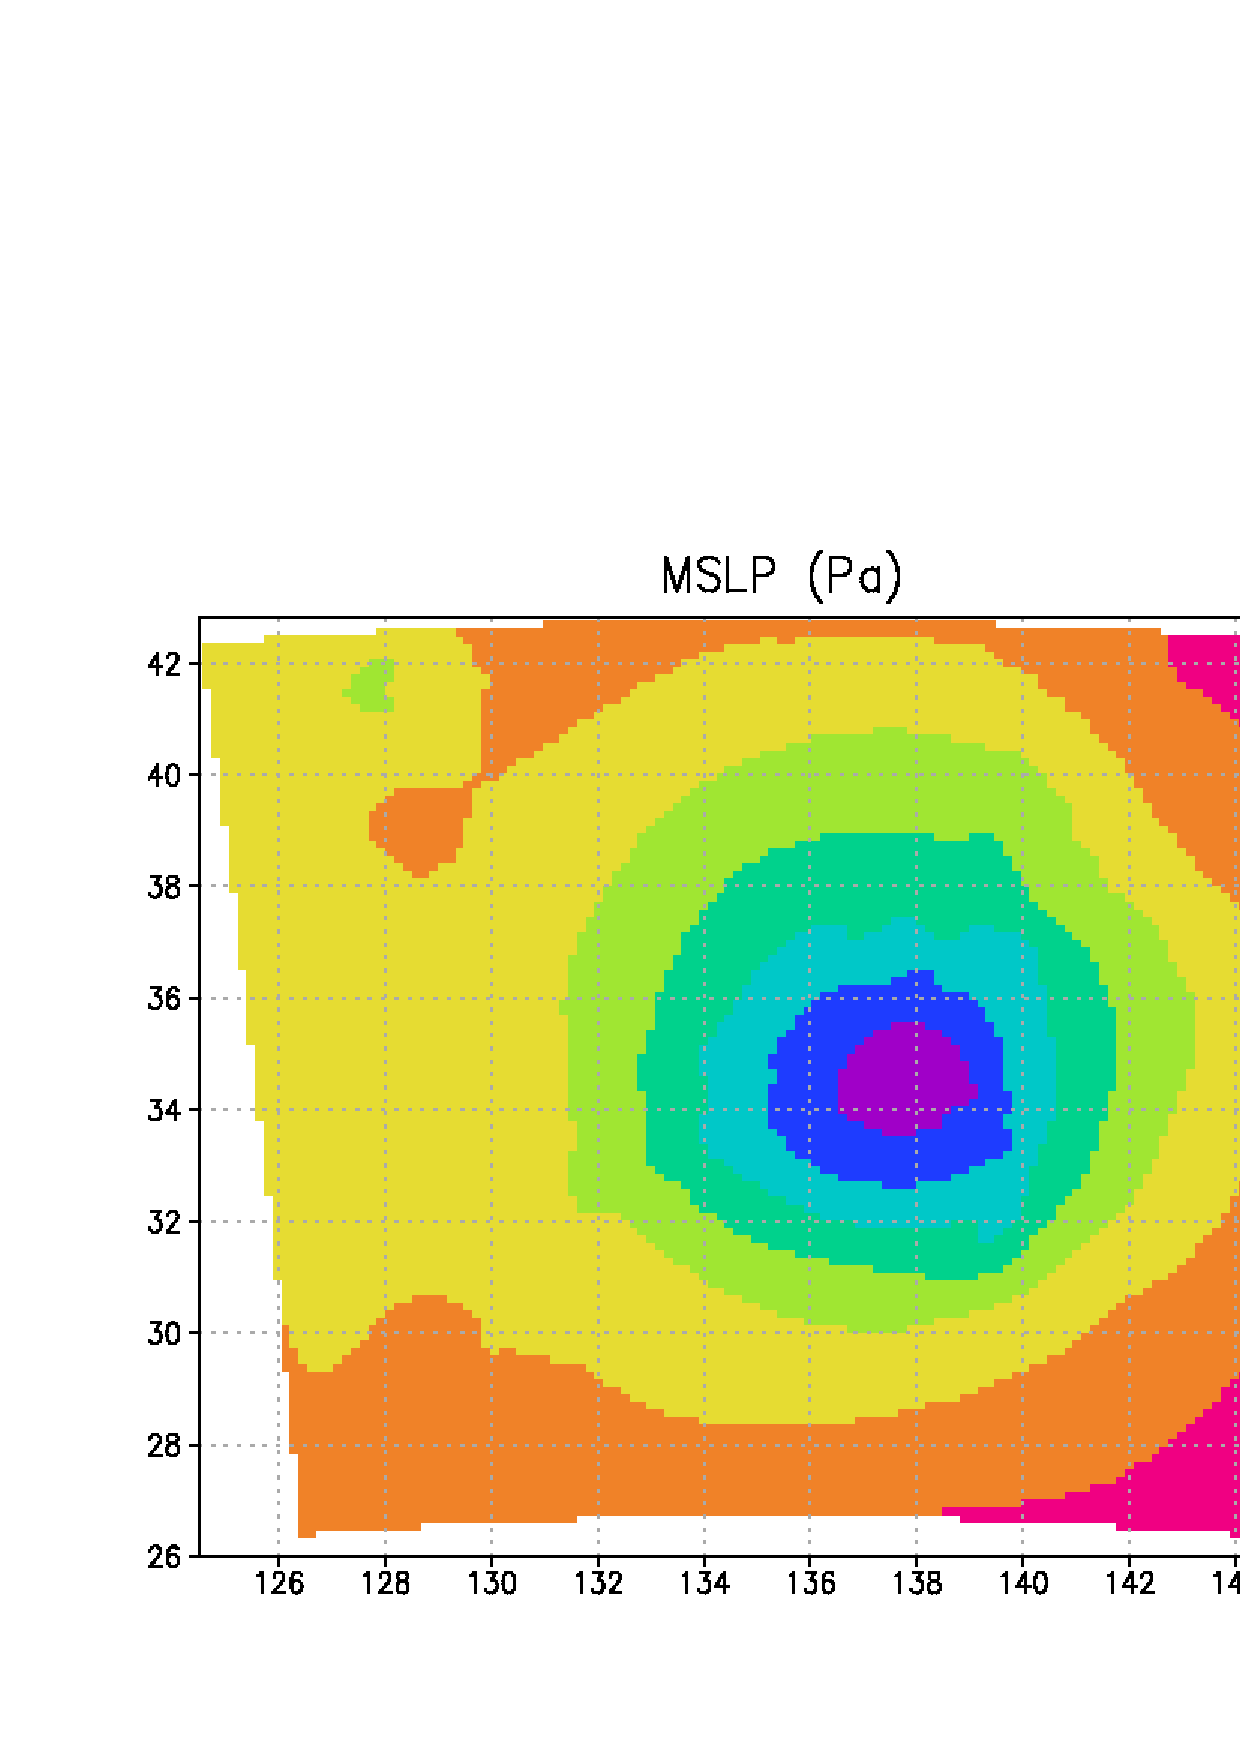
\includegraphics[width=0.55\hsize]{./../../figure/real_mslp.pdf}\\
  \caption{Sea-level pressure after 6 hours}
  \label{fig:real_mslp}
\end{center}
\begin{center}
  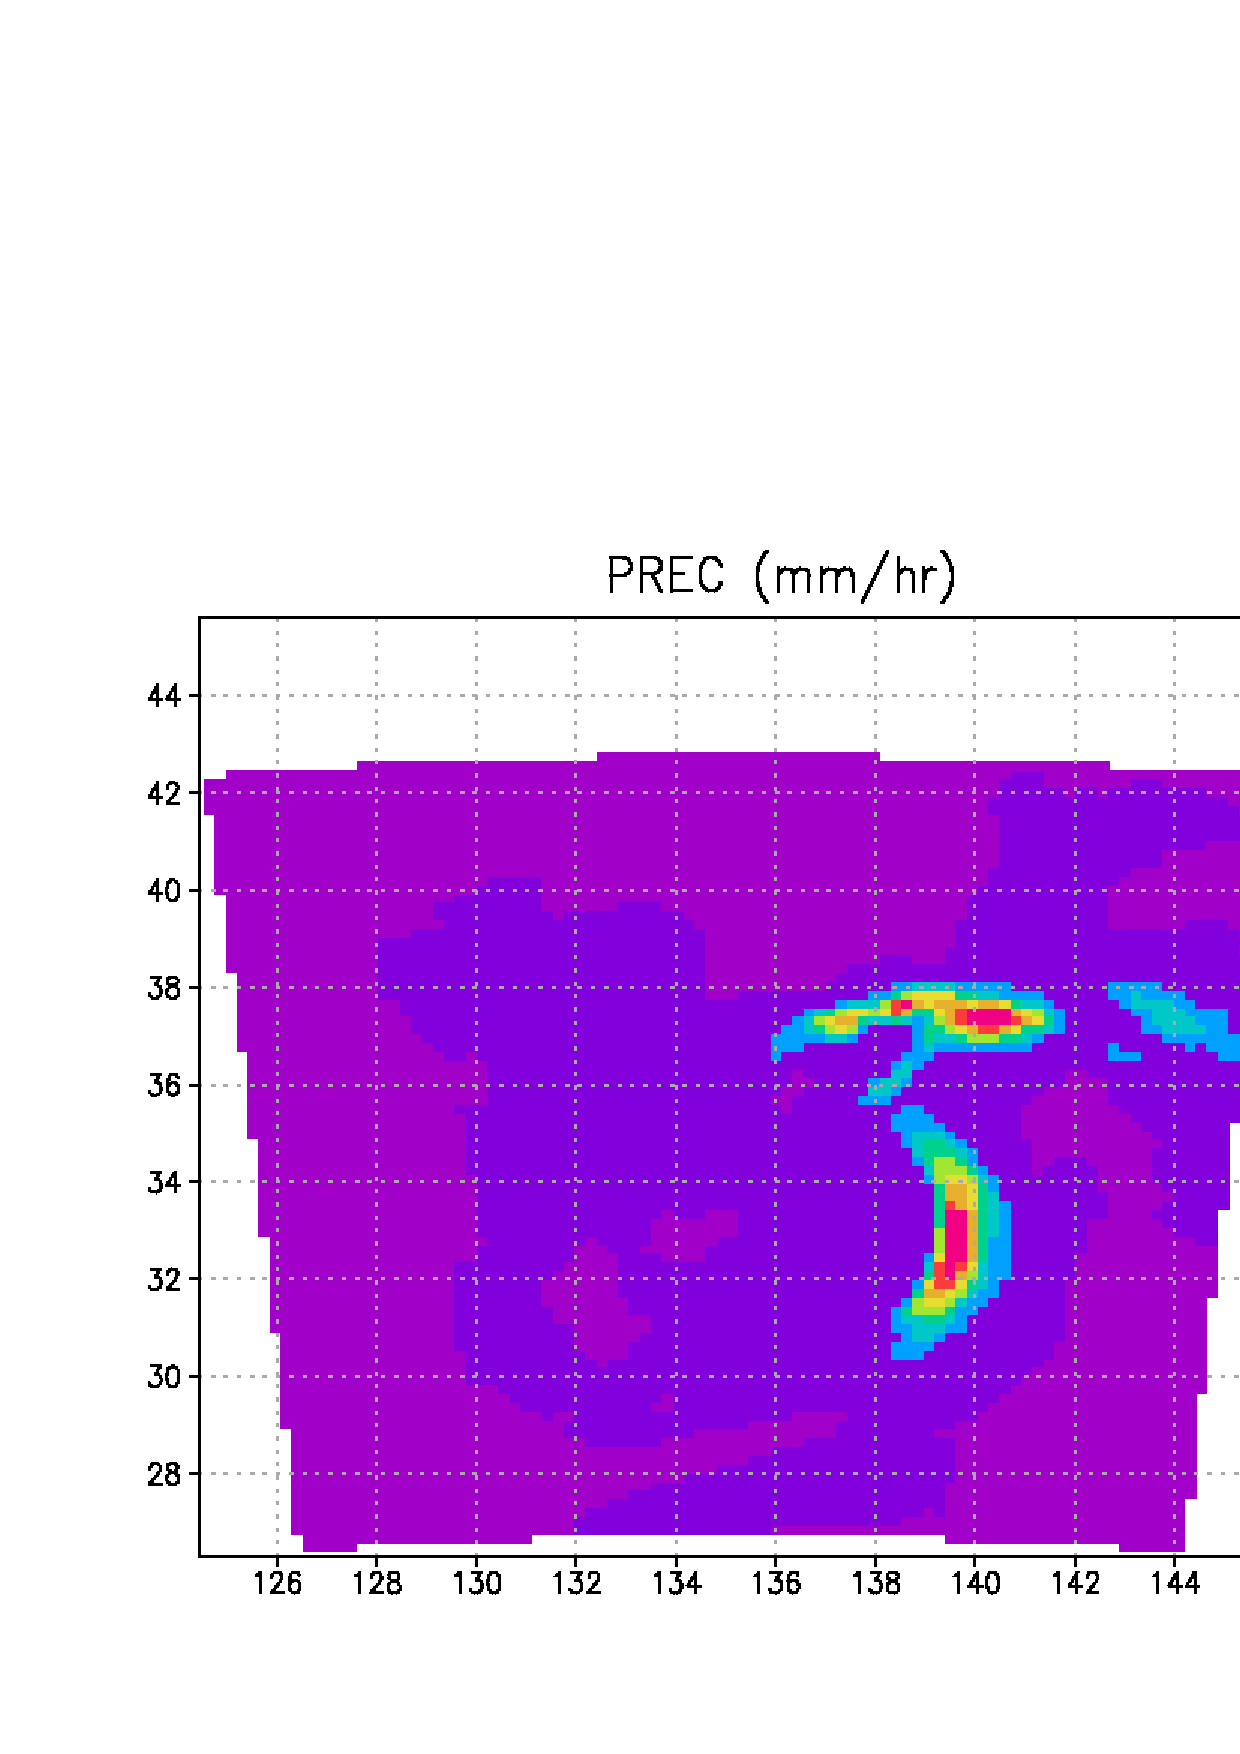
\includegraphics[width=0.55\hsize]{./../../figure/real_prec.pdf}\\
  \caption{Precipitation flux after 6 hours}
  \label{fig:real_prec}
\end{center}
\begin{center}
  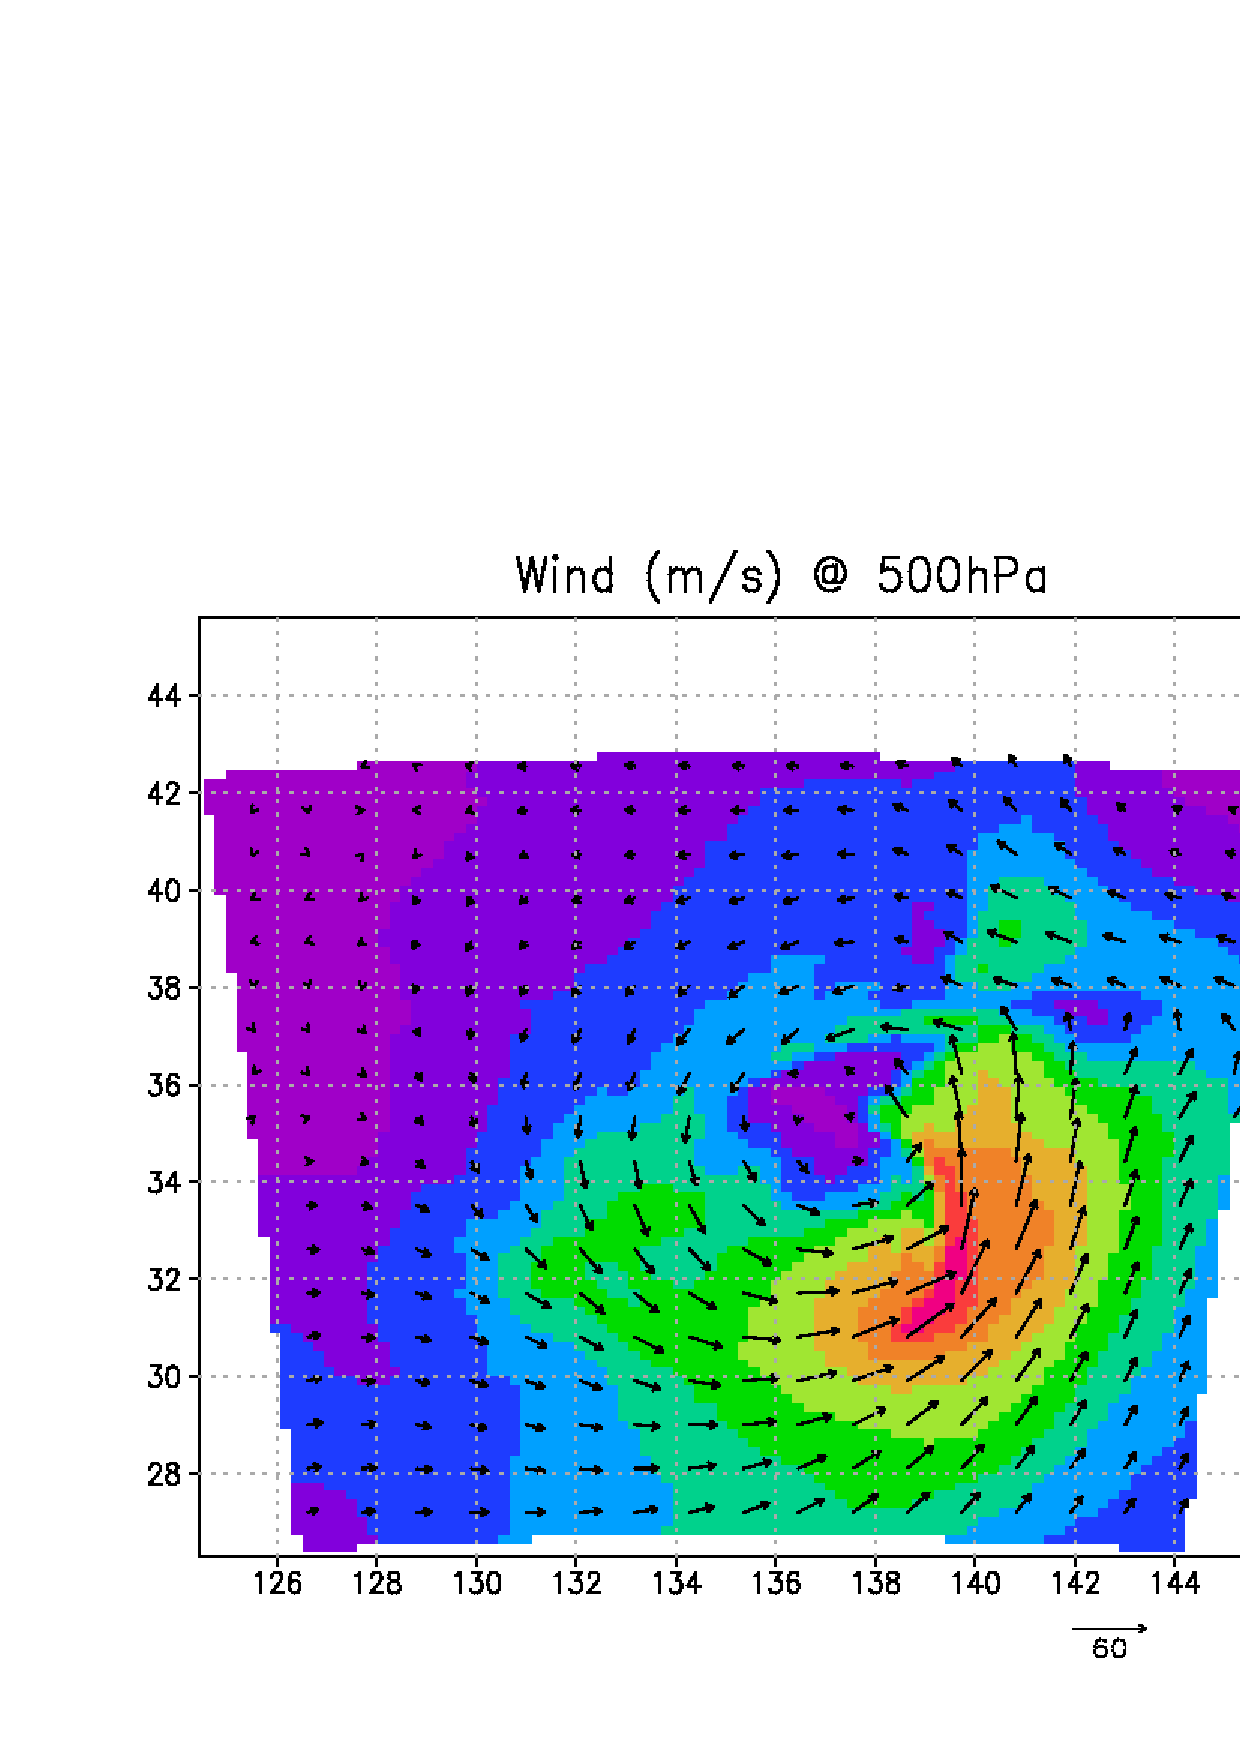
\includegraphics[width=0.55\hsize]{./../../figure/real_wind.pdf}\\
  \caption{Wind velocity after 6 hours}
  \label{fig:real_wind}
\end{center}
\end{figure}

